\documentclass[border=0pt, tikz]{standalone}
\usepackage{tikz}

\begin{document}
    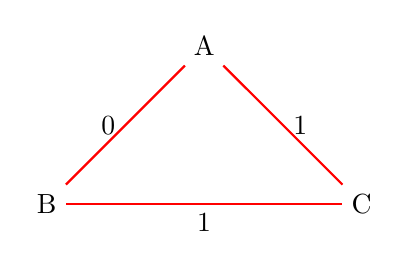
\begin{tikzpicture}[node distance = 2cm]
        \node (A) {A};
        \node [left of = A, below of = A] (B) {B};
        \node [right of = A, below of = A] (C) {C};

        \draw [thick, red] (A)--(B) node [midway, above, left] {
        \textcolor{black}0};
        \draw [thick, red] (B)--(C) node [midway, below] {\textcolor{black}1};
        \draw [thick, red] (C)--(A) node [midway, above, right] {
        \textcolor{black}1};
    \end{tikzpicture}
\end{document}
